\documentclass[a4paper, 12pt]{article}
\usepackage[utf8]{inputenc}

\usepackage[top=.25in,bottom=.25in,left=.25in,right=.25in]{geometry}
\usepackage[parfill]{parskip}
\usepackage{courier}
\usepackage{graphicx}

\usepackage{listings}
\lstset{
    frame=single,
    breaklines=true,
    basicstyle=\footnotesize\ttfamily
}

\begin{document}
\pagenumbering{gobble}

\begin{figure}[h!]
    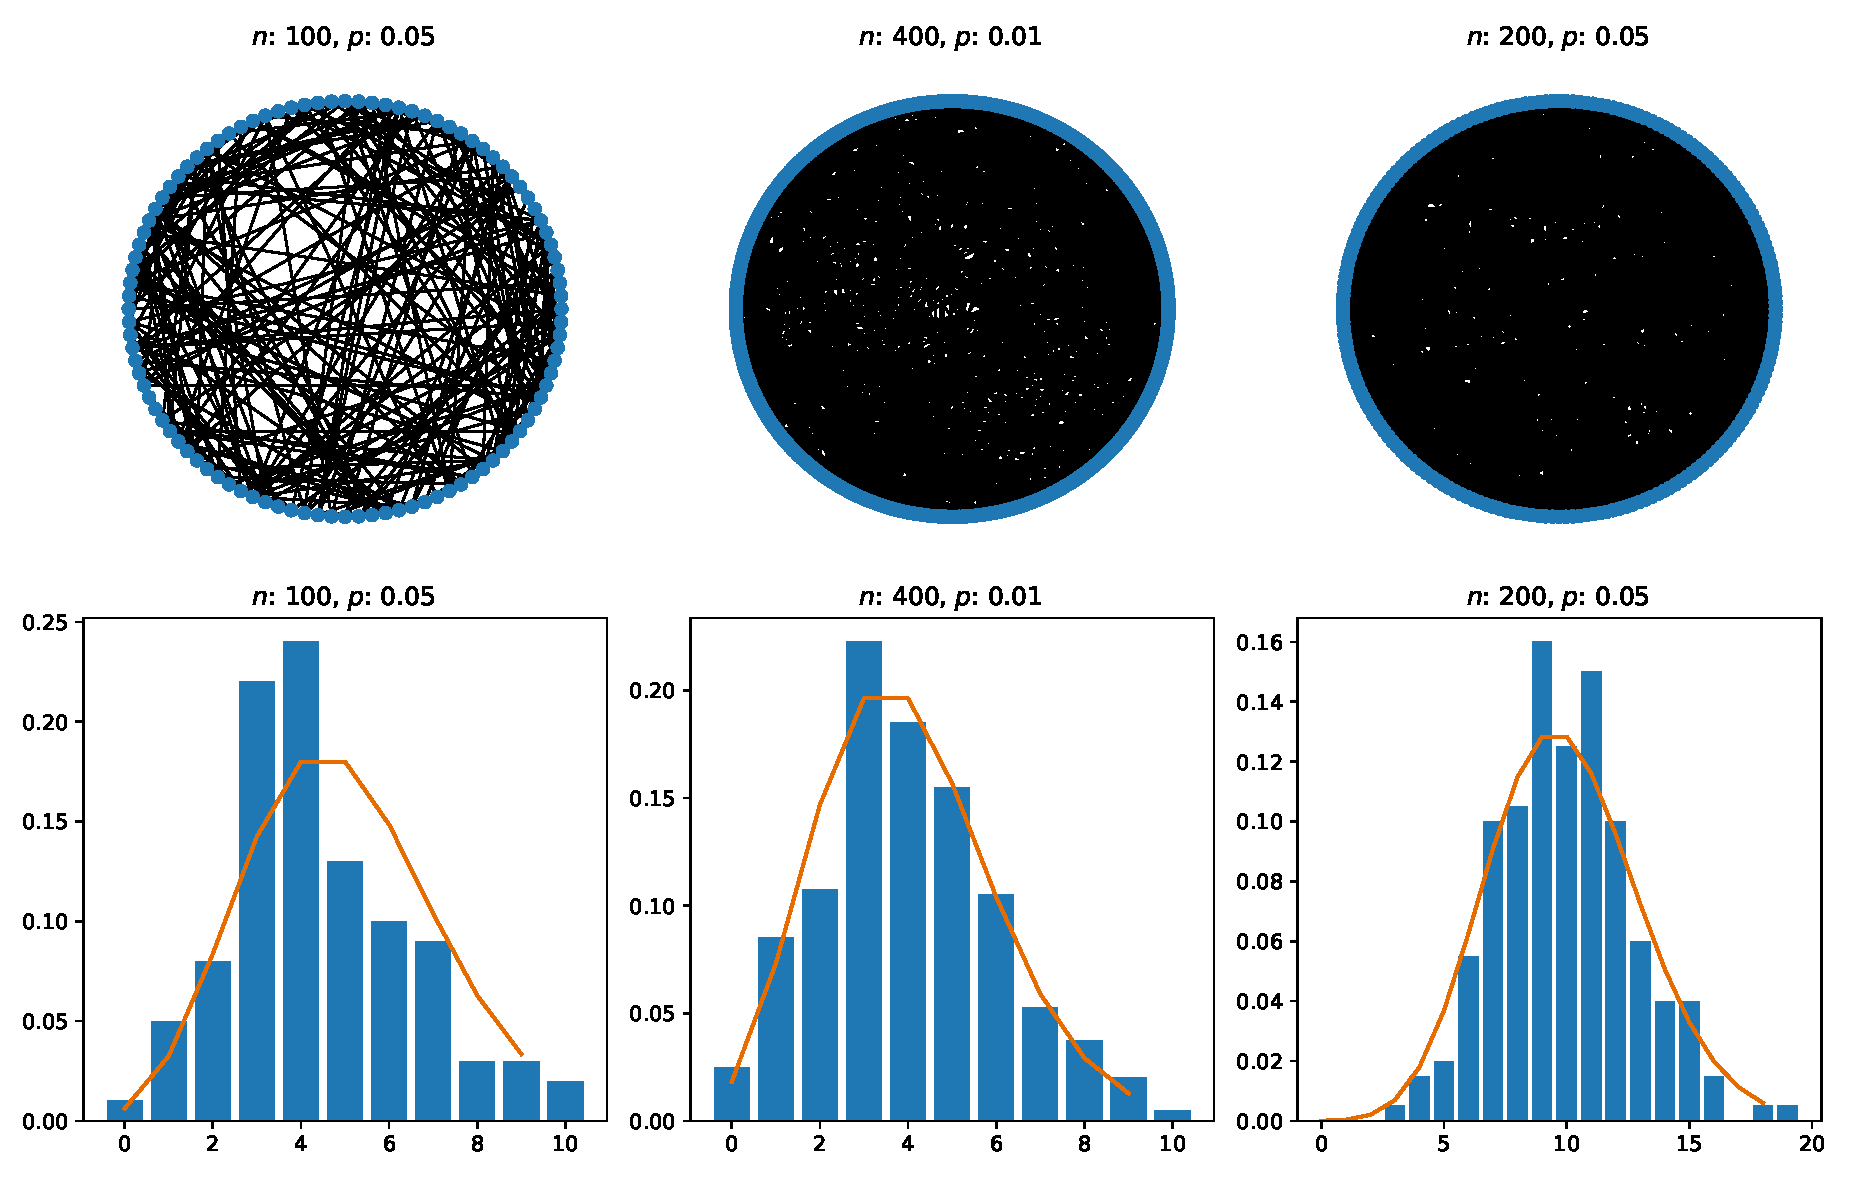
\includegraphics[width=\linewidth]{../Erdos-Renyi/erdos-reyni.pdf}
\end{figure}

\begin{figure}[h!]
    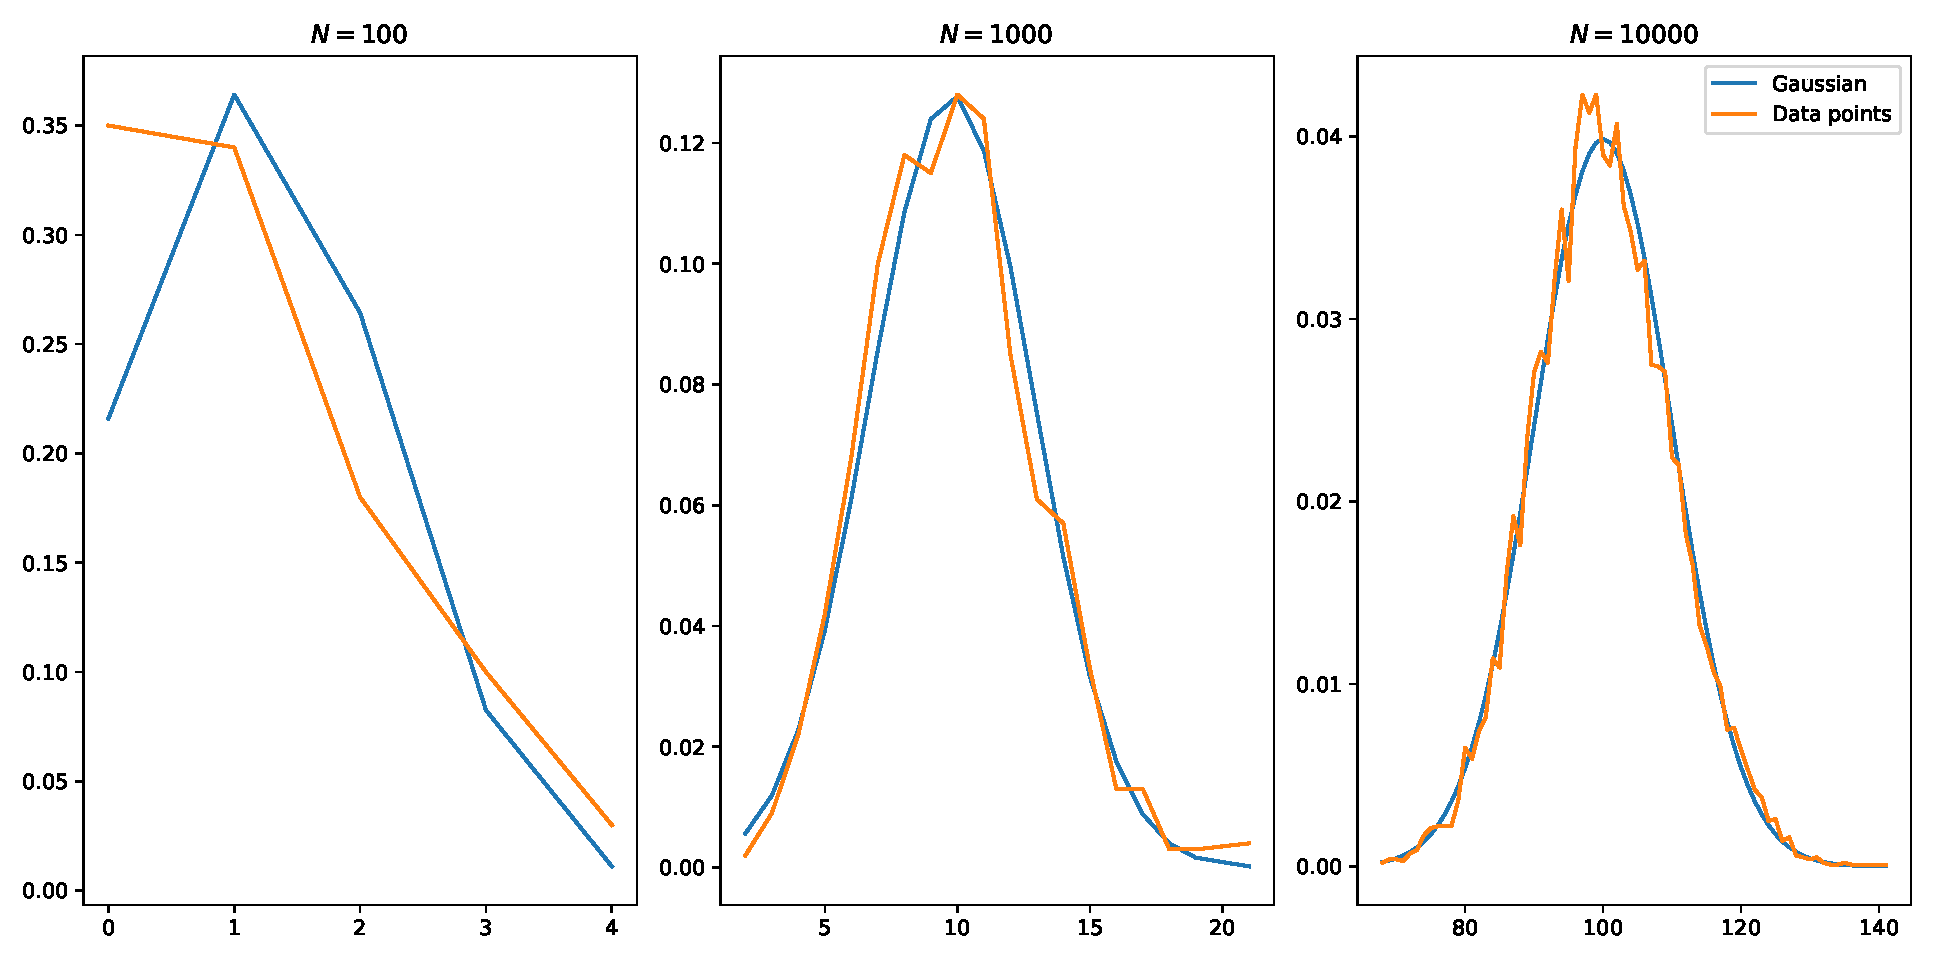
\includegraphics[width=\linewidth]{../Erdos-Renyi/gaussian.pdf}
\end{figure}

\newpage

\begin{figure}[h!]
    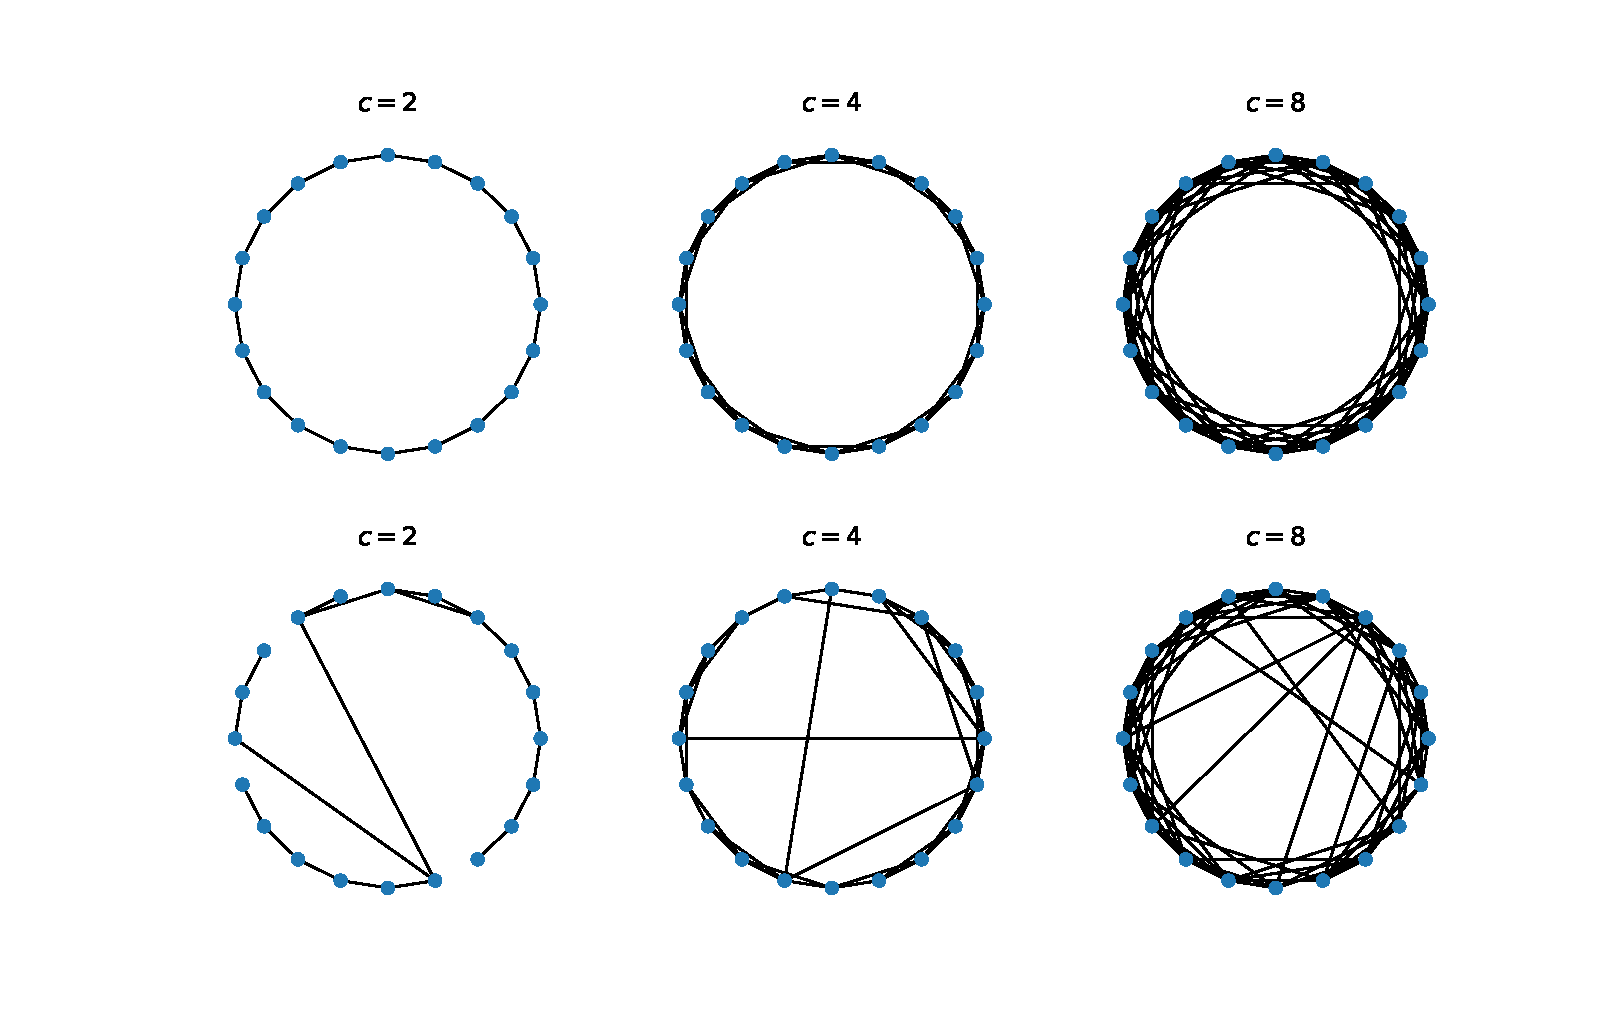
\includegraphics[width=\linewidth]{../Watts-Strogatz/c_graph.pdf}
\end{figure}

\begin{figure}[h!]
    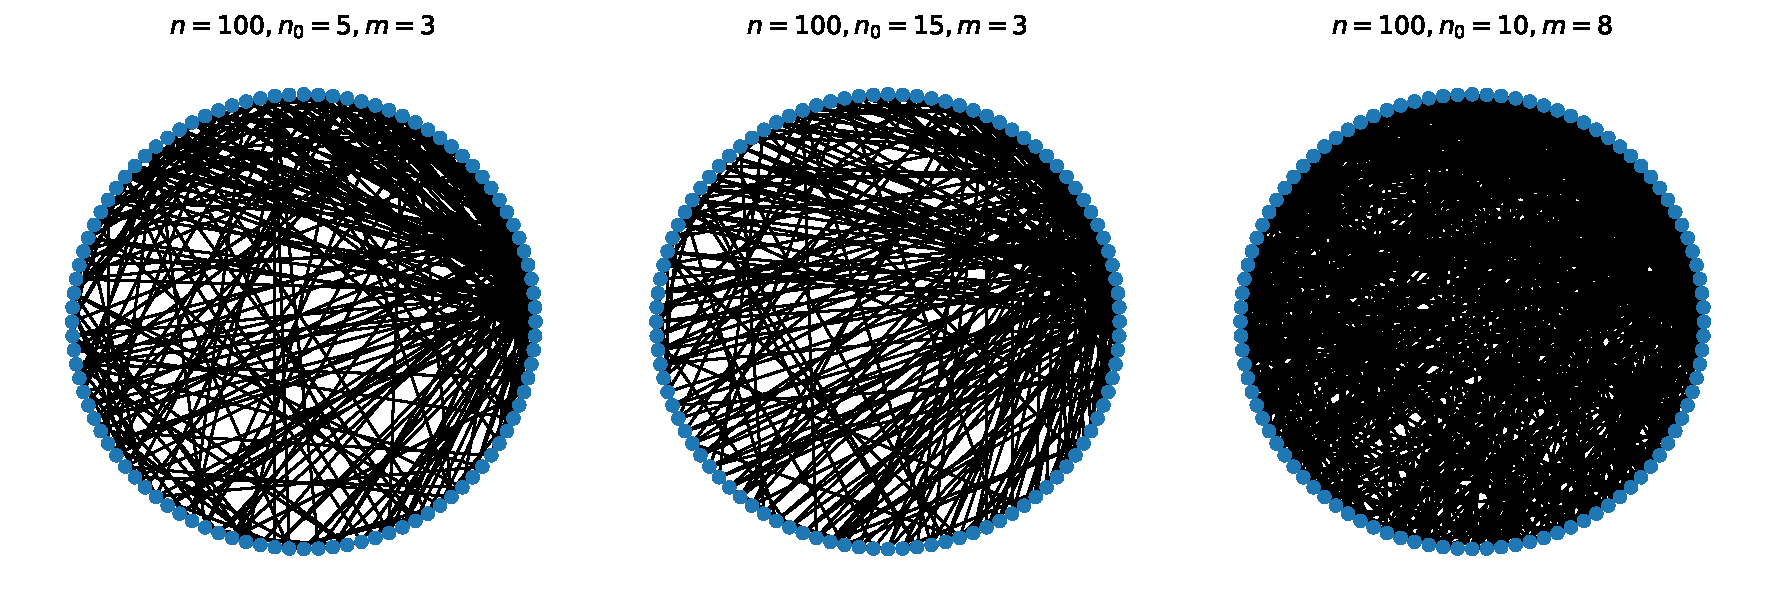
\includegraphics[width=\linewidth]{../Albert-Barabasi/graphs.pdf}
\end{figure}

\newpage

\begin{figure}[h!]
    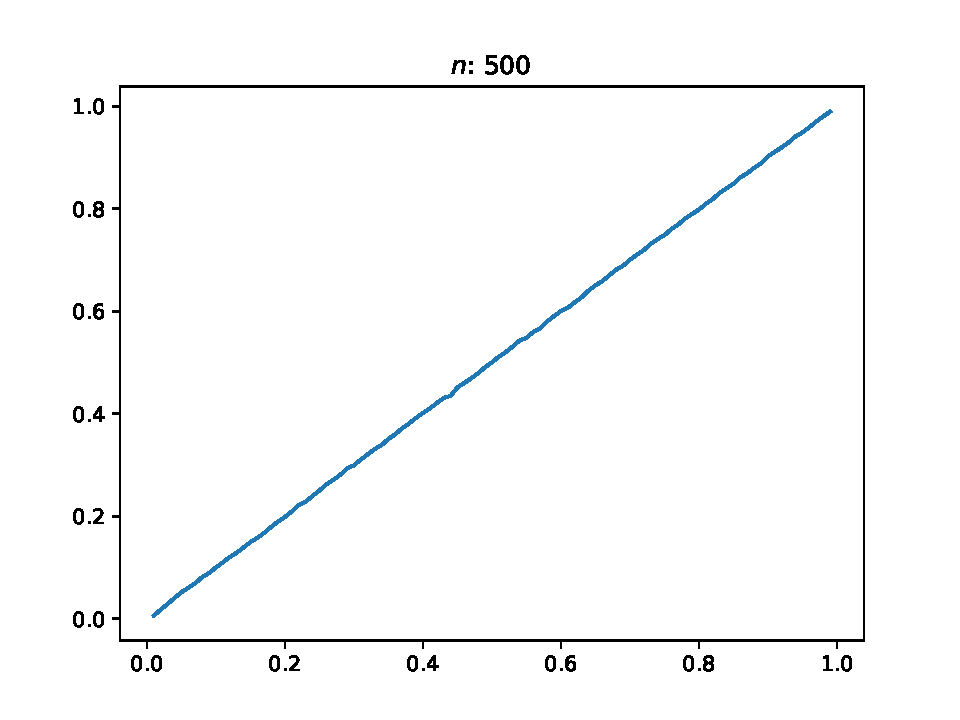
\includegraphics[width=\linewidth]{../Average-Erdos-Renyi/clustering.pdf}
\end{figure}

/Erdos-Renyi/main.py
\lstinputlisting{../Erdos-Renyi/main.py}
\newpage

/Erdos-Renyi/gaussian.py
\lstinputlisting{../Erdos-Renyi/gaussian.py}
\newpage

/Watts-Strogatz/main.py
\lstinputlisting{../Watts-Strogatz/main.py}
\newpage

/Albert-Barabasi/main.py
\lstinputlisting{../Albert-Barabasi/main.py}
\newpage

/Albert-Barabasi/dist.py
\lstinputlisting{../Albert-Barabasi/dist.py}
\newpage

/Average-Erdos-Renyi/gaussian.py
\lstinputlisting{../Average-Erdos-Renyi/main.py}
\newpage

\end{document}
